%! TEX root = 6_brace_frame.tex
% the main TeX file which is intended to compile, :VimtexReload after adjustment
   % this file should be included in the main file
% :h vimtex-tex-root
\documentclass[../modul_skb.tex]{subfiles}
%ensure the class of docs

\begin{document}

\section{Brace Frame}%
\label{sec:Brace Frame}

Struktur braced frame adalah sistem rangka bangunan yang menggunakan elemen diagonal, atau disebut bracing, untuk menahan gaya lateral yang disebabkan oleh angin atau gempa bumi. Bracing bekerja dengan cara membentuk geometri segitiga, yang secara inheren lebih kaku dan stabil dibandingkan dengan bentuk persegi panjang, sehingga mencegah deformasi atau keruntuhan struktur.

\subsection{Jenis-jenis braced frame}%
\label{sub:Jenis-jenis braced frame}

\begin{description}
	\item[Diagonal bracing]: Menggunakan satu batang diagonal di setiap bukaan rangka untuk memberikan stabilitas.
	\item[X-bracing]: Menggunakan dua batang diagonal yang saling menyilang membentuk huruf 'X'.
	\item[Inverted V-bracing (Chevron bracing)]: Menggunakan dua batang diagonal yang bertemu di tengah-tengah balok.
	\item[Eccentrically Braced Frames (EBF)]: Berbeda dari jenis konsentris, EBF didesain untuk menyalurkan gaya lateral ke area balok yang terhubung secara eksentrik (link). Area link ini dirancang untuk berdeformasi secara daktail (liat) saat terjadi gempa besar, sehingga menyerap energi dan mencegah kegagalan pada bagian struktur lainnya.
	\item[Concentric Braced Frames (CBF)]: Jenis braced frame di mana garis aksi semua elemen bracing berpotongan di satu titik, biasanya pada sambungan balok-kolom.
\end{description}

\begin{figure}
	\begin{center}
		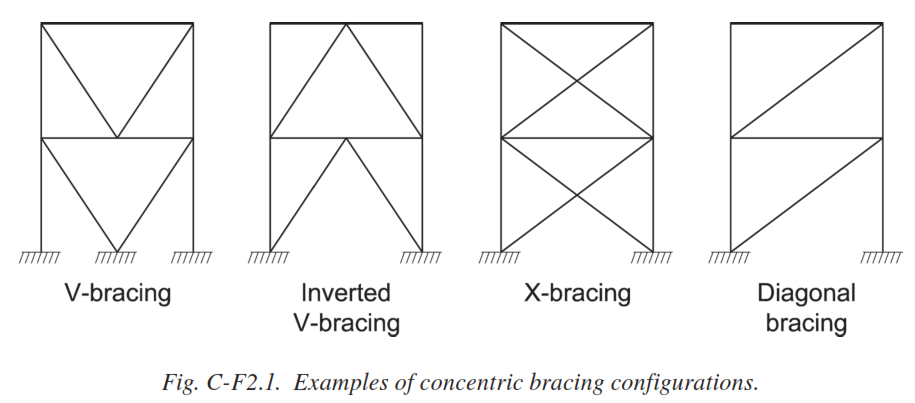
\includegraphics[width=.82\textwidth]{../figures/bracing_frame.png}
		% filename may not contain space but _
	\end{center}
	\caption{Macam-macam Rangka Brace}
	\label{fig:brace}
\end{figure}


\subsection{Kelebihan Sistem Braced Frame}%
\label{sub:Kelebihan Sistem Braced Frame}

\begin{enumerate}
	\item Memiliki kekakuan lateral yang tinggi. Bracing sangat efektif dalam menahan gaya gempa dan angin sehingga simpangan (drift) bangunan dapat berkurang.
	\item Lebih efisien dibandingkan \textit{rigid frame}. Pada bangunan tinggi, penggunaan material menjadi lebih hemat karena tidak hanya mengandalkan kekakuan sambungan balok–kolom.
	\item Proses konstruksi relatif cepat. Jika menggunakan bracing baja, pemasangan dapat dilakukan melalui metode fabrikasi dan erection di lapangan.
	\item Meringankan beban pada kolom dan balok. Beban lateral ditahan oleh sistem bracing, sehingga elemen kolom dan balok dapat dirancang lebih ringan.
	\item Fleksibel dalam konfigurasi. Sistem ini dapat menggunakan berbagai pola seperti X-brace, K-brace, V-brace, Chevron, atau Diagrid sesuai kebutuhan arsitektur dan struktur.
\end{enumerate}

\subsection{Kekurangan Sistem Braced Frame:}%
\label{sub:Kekurangan Sistem Braced Frame:}

\begin{enumerate}
	\item Mengurangi fleksibilitas arsitektur. Kehadiran batang diagonal dapat menutup jendela, mengganggu estetika, atau membatasi tata ruang interior.
	\item Rentan terhadap buckling. Batang bracing bekerja dalam kondisi tarik–tekan; pada kondisi tekan, bracing baja berpotensi mengalami tekuk (buckling) jika tidak dirancang dengan baik.
	\item Perawatan lebih rumit pada baja. Jika menggunakan bracing baja, terutama yang terekspos di luar bangunan, diperlukan perlindungan terhadap korosi serta perawatan berkala.
\end{enumerate}

\section{Outrrigger}%
\label{sec:Outrrigger}

Struktur outrigger adalah sistem struktural yang kaku dan horizontal, digunakan pada gedung-gedung tinggi dan mesin-mesin berat untuk memberikan stabilitas dan menahan gaya-gaya yang kuat. Pada gedung tinggi, outrigger memindahkan gaya guling yang besar dari inti pusat ke kolom-kolom perimeter eksterior gedung, secara efektif menguatkan seluruh struktur terhadap beban angin dan seismik.

\subsection{Cara kerja struktur outrigger}%
\label{sub:Cara kerja struktur outrigger}
Pada gedung bertingkat tinggi, gaya lateral dari angin atau gempa bumi dapat menyebabkan gedung bergoyang atau "bergeser" (drift) dan dapat menciptakan momen guling yang besar pada inti pusat. Tanpa outrigger, inti bertindak seperti cantilever yang berdiri bebas, dengan semua resistansi berasal dari dasarnya sendiri. Outrigger mengubah ini dengan cara:


\begin{description}
	\item[Menghubungkan inti dan kolom:] Struktur outrigger, yang sering kali berupa truss atau dinding beton, berfungsi sebagai balok yang kaku dan dalam yang menghubungkan inti pusat gedung yang kaku (yang biasanya berisi elevator dan tangga) dengan kolom-kolom di perimeter
	\item[Menciptakan pasangan gaya penstabil:] Ketika inti gedung mencoba membengkok dan berputar di bawah beban lateral, outrigger akan melibatkan kolom-kolom
	\item[Mengurangi gaya guling:] Tindakan ini menciptakan pasangan gaya penstabil yang kuat yang secara signifikan mengurangi momen guling pada inti dan dasar gedung, membuat keseluruhan struktur menjadi jauh lebih kaku dan stabil. Hal ini juga mengurangi goyangan lateral, atau pergeseran, di bagian atas gedung, sehingga meningkatkan kenyamanan penghuni.
\end{description}

Sistem struktur outrigger memiliki keunggulan yang signifikan dalam meningkatkan stabilitas dan kekuatan bangunan tinggi, terutama dalam menghadapi beban lateral seperti angin dan gempa bumi. Namun, sistem ini juga datang dengan beberapa tantangan dan keterbatasan yang perlu dipertimbangkan.

\begin{figure}
	\begin{center}
		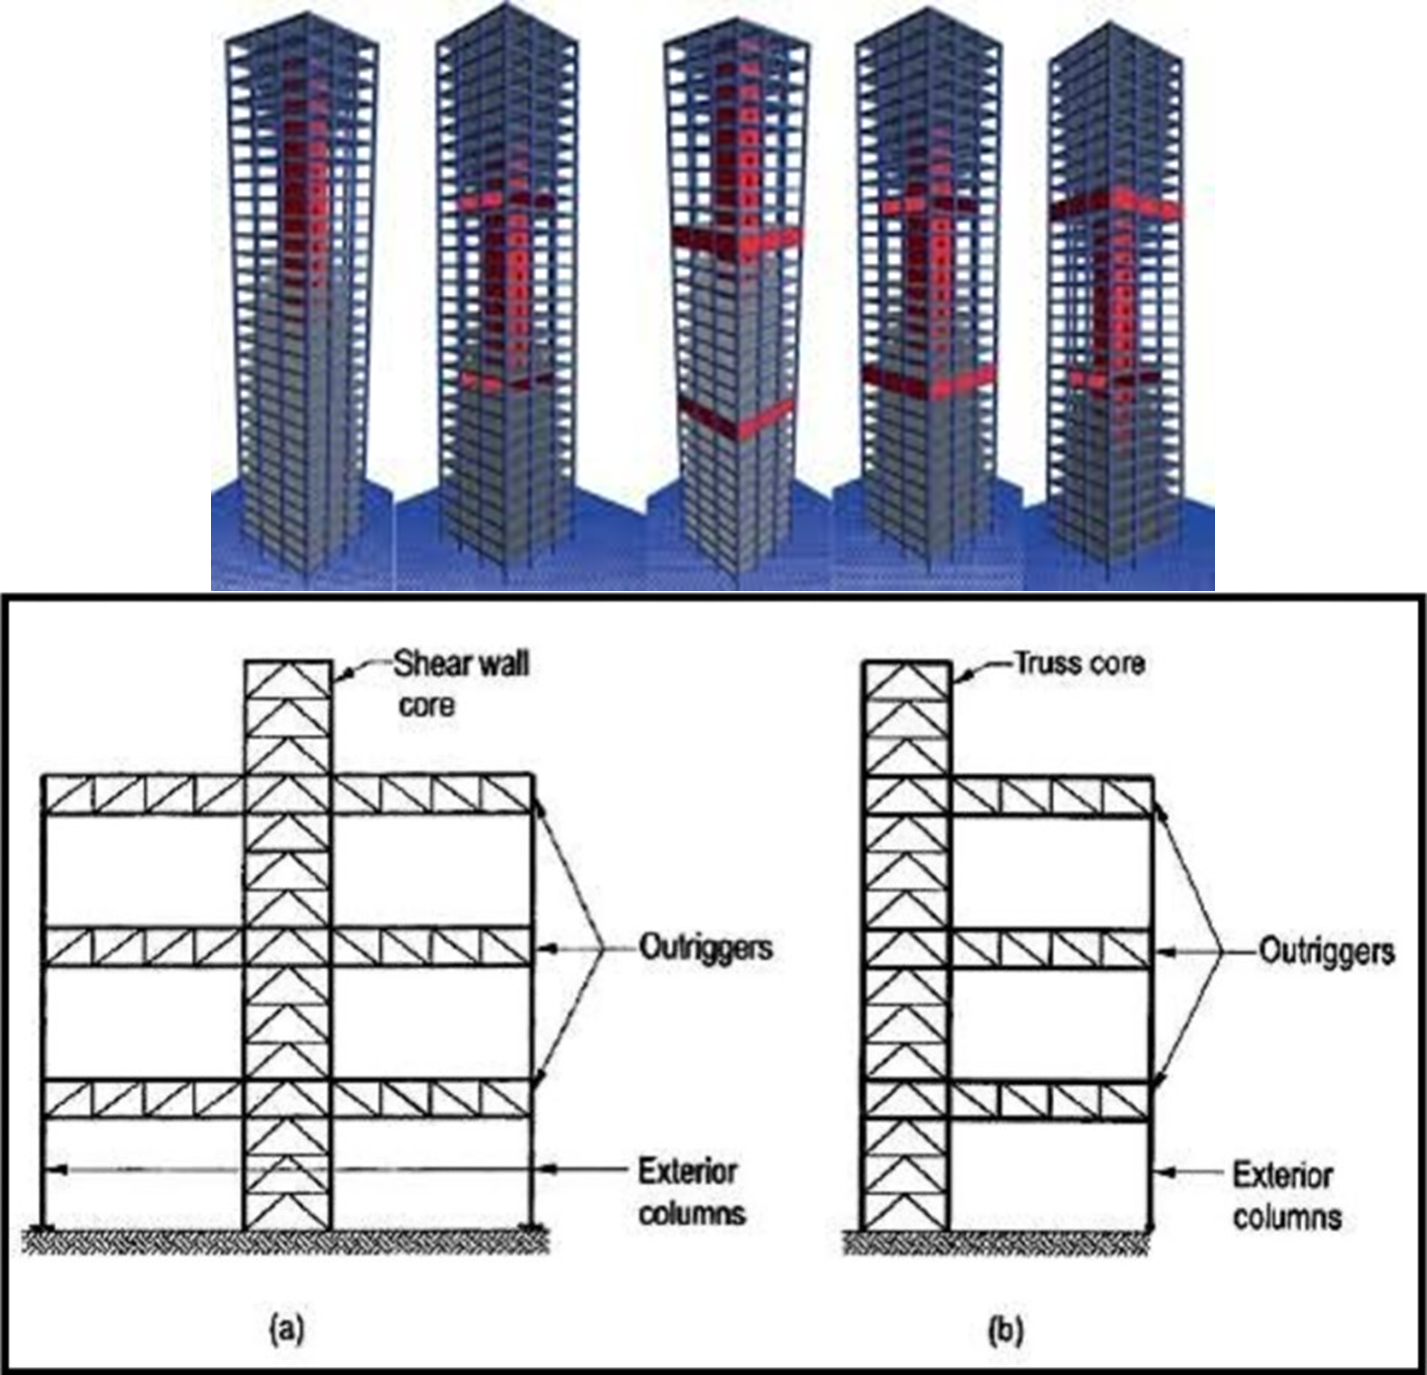
\includegraphics[width=.82\textwidth]{../figures/outriggers.png}
		% filename may not contain space but _
	\end{center}
	\caption{Outriggers}
	\label{fig:outriggers_frame}
\end{figure}

\subsection{Kelebihan Outriggers}%
\label{sub:Kelebihan Outriggers}

\begin{itemize}
	\item Peningkatan Kekakuan Lateral: Dengan menghubungkan inti (core) bangunan dengan kolom-kolom luar, sistem ini secara efektif meningkatkan kekakuan seluruh struktur, sehingga mengurangi simpangan lateral (drift) akibat beban angin atau gempa.
	\item Pengurangan Momen Guling: Outrigger menggerakkan kolom-kolom eksterior untuk menciptakan pasangan gaya yang bekerja melawan momen guling pada inti, sehingga secara signifikan mengurangi beban pada pondasi inti.
	\item Efisiensi Material: Karena outrigger mengurangi momen guling yang harus ditahan oleh inti, dimensi inti dan pondasi bisa dibuat lebih ekonomis. Desain ini sering kali memungkinkan penggunaan material yang lebih efisien.
	\item Fleksibilitas Arsitektural: Penggunaan outrigger dapat memungkinkan perancang untuk menggunakan kolom-kolom luar yang lebih sederhana tanpa harus memiliki sambungan yang kaku, yang bisa mengarah pada solusi yang lebih ekonomis.
	\item Peningkatan Kenyamanan Penghuni: Dengan mengurangi goyangan di puncak gedung, outrigger membantu meningkatkan kenyamanan bagi penguni, terutama di lantai atas saat terjadi angin kencang.
\end{itemize}

\subsection{Kekurangan Outriggers}%
\label{sub:Kekurangan Outriggers}

\begin{itemize}
	\item Gangguan Ruang: Pemasangan outrigger truss yang besar, terutama yang menggunakan elemen diagonal, dapat memakan banyak ruang pada lantai tempat ia dipasang. Hal ini dapat mengganggu fungsi ruang dan aspek arsitektural bangunan.
	\item Kompleksitas Konstruksi: Menghubungkan outrigger dengan inti (misalnya, shear wall beton) bisa menjadi proses yang rumit, terutama jika inti dan outrigger terbuat dari material yang berbeda. Proses ini membutuhkan ketelitian tinggi.
	\item Masalah Pemendekan Diferensial: Inti dan kolom-kolom luar mungkin mengalami pemendekan yang tidak sama akibat beban gravitasi. Outrigger harus didesain sangat kaku untuk mengatasi masalah ini, yang dapat meningkatkan gaya pada struktur jika pemendekan tidak diperhitungkan dengan cermat.
	\item Masalah Fungsional: Masalah arsitektural dan fungsional dapat muncul karena keberadaan outrigger yang terhubung ke inti, terutama jika letaknya berada di area yang penting secara fungsional.
	\item Tidak Selalu Optimal: Lokasi pemasangan outrigger yang paling efektif untuk mengurangi simpangan lateral mungkin tidak selalu tersedia karena pertimbangan arsitektural atau fungsional. Efektivitas sistem sangat bergantung pada lokasi dan kekakuan outrigger.
\end{itemize}


\section{Belt Truss}%
\label{sec:Belt Truss}

Belt truss adalah sistem struktur rangka batang yang kaku dan dipasang secara horizontal melingkari bagian luar bangunan tinggi. Fungsi utamanya adalah untuk mengikat kolom- kolom eksterior bangunan ke inti (core wall) agar struktur dapat menahan beban lateral yang disebabkan oleh angin dan gempa bumi dengan lebih baik.

Pada dasarnya, sistem ini bekerja bersama dengan sistem outrigger atau inti kaku (core wall) untuk mengendalikan pergerakan atau goyangan (simpangan lateral) pada bagian atas gedung.

\begin{figure}
	\begin{center}
		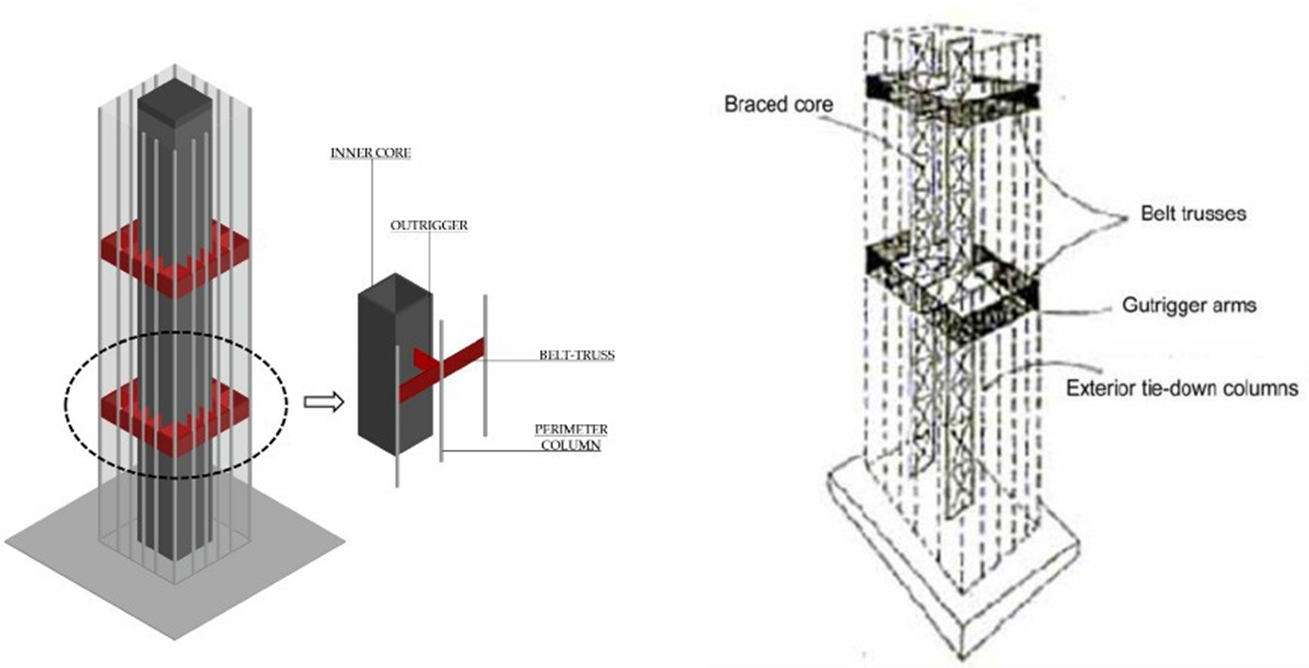
\includegraphics[width=.82\textwidth]{../figures/belt_truss.png}
		% filename may not contain space but _
	\end{center}
	\caption{Belt Truss}
	\label{fig:belt_truss}
\end{figure}


\subsection{Ciri-ciri Belt Truss}%
\label{sub:Ciri-ciri Belt Truss}

\begin{description}
	\item[Melindungi inti bangunan (core wall):] Gaya lateral yang diterima inti bangunan akan disalurkan ke kolom eksterior melalui belt truss, sehingga mengurangi momen guling yang diterima inti.
	\item[Menggunakan berbagai material:] Belt truss dapat dibuat dari material baja, beton bertulang, atau kombinasi keduanya (komposit).
	\item[Lokasi penempatan strategis:] Penempatannya biasanya berada pada lantai-lantai mekanikal atau lantai penyelamatan (refuge floor) pada bangunan tinggi. Lokasi penempatan yang optimal, seperti pada bagian atas dan tengah bangunan, dapat meningkatkan efektivitasnya dalam mereduksi simpangan lateral.
	\item[Menghubungkan inti dan kolom eksterior:] Belt truss secara efektif menghubungkan kolom-kolom terluar (fasade) dengan inti bangunan yang berisi lift atau tangga darurat.
\end{description}

\subsection{Kelebihan Belt Truss}%
\label{sub:Kelebihan Belt Truss}


\begin{itemize}
	\item Mengurangi simpangan lateral: Pemasangan belt truss dapat mengurangi pergerakan horizontal (simpangan lateral atau drift) akibat beban angin dan gempa bumi hingga 25\%–35\%.
	\item Meningkatkan kekakuan struktur: Sistem ini secara signifikan meningkatkan kekakuan total bangunan, membuat gedung lebih stabil dan aman.
	\item Efektif untuk bangunan tidak simetris: Sistem belt truss sangat efektif untuk mengurangi gerakan memutar (torsional movement) pada bangunan yang memiliki denah tidak simetris.
	\item Mengoptimalkan distribusi beban: Belt truss membantu mendistribusikan beban lateral secara merata dari inti ke seluruh kolom eksterior, sehingga kolom menahan gaya aksial (tarik atau tekan) dan mengurangi tegangan pada inti.
\end{itemize}
\subsection{Kekurangan Belt Truss}%
\label{sub:Kekurangan Belt Truss}
\begin{itemize}
	\item Keterbatasan arsitektur: Kehadiran belt truss dapat mengganggu tata letak lantai dan desain interior karena elemen-elemen rangka harus ditempatkan pada level tertentu. Ini dapat membatasi penataan ruang, terutama jika diletakkan di lantai yang sering digunakan.
	\item Konstruksi yang rumit: Pemasangan dan sambungan belt truss membutuhkan keahlian khusus dan perencanaan yang matang. Pemasangan yang tidak presisi dapat mengurangi efektivitasnya.
	\item Biaya yang lebih tinggi: Sistem ini menambah biaya konstruksi, terutama karena penggunaan material tambahan dan kompleksitas dalam perancangan serta instalasi.
	\item Mengganggu sistem mekanikal: Penempatan belt truss sering kali harus disesuaikan dengan sistem mekanikal, elektrikal, dan pipa (MEP) yang sudah ada, yang bisa memakan ruang dan menyebabkan konflik dalam perencanaan.
\end{itemize}






\bibliographystyle{apalike}
\bibliography{../filename.bib} % required for citecompletion, not work in mainfile
\end{document}

